%
% $Id: $
%
%
% Compilar a .pdf con LaTeX (pdflatex)
% Es necesario instalar Beamer (paquete latex-beamer en Debian)
%

%
% Gráficos:
% Los gráficos pueden suministrarse en PNG, JPG, TIF, PDF, MPS
% Los EPS deben convertirse a PDF (usar epstopdf)
%

\documentclass{beamer}
\usetheme{Warsaw}
\usebackgroundtemplate{
\includegraphics[width=\paperwidth]{format/libresoft-bg-soft.png}}
% \usepackage[spanish]{babel}
\usepackage[utf8]{inputenc}
\usepackage{graphics}
\usepackage{amssymb} % Simbolos matematicos

%\definecolor{libresoftgreen}{RGB}{162,190,43}
%\definecolor{libresoftblue}{RGB}{0,98,143}

%\setbeamercolor{titlelike}{bg=libresoftgreen}

%% Metadatos del PDF.
\hypersetup{
  pdftitle={An Introduction to GNU R},
  pdfauthor={Felipe Ortega},
  pdfcreator={GSyC/LibreSoft, Universidad Rey Juan Carlos},
  pdfproducer=PDFLaTeX,
  pdfsubject={Case studies I},
}
%%

\begin{document}

\title{An Introduction to GNU R}
\subtitle{Case studies I / Master on libre software (URJC) \\
\url{http://master.libresoft.es}}
\author{Felipe Ortega}
\institute{jfelipe@libresoft.es \\
\url{http://identi.ca/jfelipe} \url{http://twitter.com/jfelipe} \\
GSyC/LibreSoft, Universidad Rey Juan Carlos}

\date{September 2011}

\frame{
\maketitle
\begin{center}

\includegraphics[width=6cm]{format/gsyc-urjc}
\end{center}
}


% Si el titulo o el autor se quieren acortar para los pies de página
% se pueden redefinir aquí:
%\title{Titulo corto}
%\author{Autores abreviado}


%% LICENCIA DE REDISTRIBUCION DE LAS TRANSPAS
\frame{
~
\vspace{3cm}

\begin{flushright}
\copyright 2010-2011 Felipe Ortega. \\

Some rights reserved. \\
This document is distributed under the \\
Creative Commons Attribution-ShareAlike 3.0 licence, \\
available in \\
\url{http://creativecommons.org/licenses/by-sa/3.0}

The original version of this document is available at \\
\url{http://master.libresoft.es}
\end{flushright}
}
%%

%%%%%%%%%%%%%%%%%%%%%%%%%%%%%%%%%%%%%%%%%%%%%%%%%%%%%%%%%%%%%%%%%%%%%%%

\begin{frame}

\frametitle{What is R?}
\begin{itemize}
\item Language and environment for statistical computing and graphics.
\item Powerful, easy-to-use and \textit{libre software} (GNU GPL v2).
\item Created by Ross Ihaka and Robert Gentleman, based on S language created by Chambers et al. (Bell Labs).
\item It is a GNU project, now maintained by the \textit{R Development Core Team}.
\item Available for multiple operating systems.
\end{itemize}

\begin{flushright}
 \url{http://www.r-project.org/}
\end{flushright}


\end{frame}

%%%%%%%%%%%%%%%%%%%%%%%%%%%%%%%%%%%%%%%%%%%%%%%%%%%%%%%%%%%%%%%%%%%%%%%

\begin{frame}

\frametitle{Why do we introduce R?}
\begin{itemize}
\item It has become the \textit{de facto} standard for statistical computing.
\item Companies using R: Google, Pfizer, Merck, Johnson \& Johnson, Shell, Bank of America, etc.
\item R is \textit{extensible} (libraries or writing your own code/functions).
\item R CRAN: 3,305 packages available (1,600 in Jan. 2009, exp. growth).
\item You will use R to perform data analysis, create graphs and reports.
\end{itemize}

\begin{flushright}
 \url{http://cran.es.r-project.org/}
\end{flushright}

\end{frame}

%%%%%%%%%%%%%%%%%%%%%%%%%%%%%%%%%%%%%%%%%%%%%%%%%%%%%%%%%%%%%%%%%%%%%%%

\begin{frame}

\frametitle{Installation}
 \begin{itemize}
  \item Installing R with Debian packages:
  \begin{enumerate}
   \item \texttt{fenix@blackstorm:\~\$ sudo aptitude update}
   \item \texttt{fenix@blackstorm:\~\$ sudo aptitude install r-base r-cran-rmysql}
   \item Other useful packages: \texttt{r-cran-lattice r-cran-latticeextra r-cran-hmisc}...
  \end{enumerate}
   \item To start R just type in the command-line:\\
     \texttt{fenix@blackstorm:\~ \$ R}\\
     \texttt{[...]}\\
     \texttt{>}\\
    You are now in the R environment, with its own command-line.
 \end{itemize}

\end{frame}

%%%%%%%%%%%%%%%%%%%%%%%%%%%%%%%%%%%%%%%%%%%%%%%%%%%%%%%%%%%%%%%%%%%%%%%

\begin{frame}

\frametitle{Getting Help}
  R command-line:
  \begin{enumerate}
   \item Help about functions (usage, args...).\\
   \texttt{> help(funcName)}\\
   \texttt{> ?funcName} 
   \item Search through help doc\\
   \texttt{help.search(``word'')}\\
   \texttt{> apropos(''word'')}.
   \item What is inside a library?\\
   \texttt{> library(help=MASS)}
   \end{enumerate}
  Manual: ``An Introduction to R'' \url{http://cran.r-project.org/doc/manuals/R-intro.pdf}

\end{frame}

%%%%%%%%%%%%%%%%%%%%%%%%%%%%%%%%%%%%%%%%%%%%%%%%%%%%%%%%%%%%%%%%%%%%%%%

\begin{frame}

 \frametitle{R libraries}
 \begin{itemize}
  \item Packages that provide collections of functions
  and data sets.
  \item Best solution to perform many statistical
 analyses.\\
  \texttt{library(``libnName'') \#Load library}\\
  Example:\\
  \texttt{> library(MASS)}\\
  Install libraries: (execute R with sudo)\\
  \texttt{> install.packages(``ISwR'', dep=T)}\\
  Select the mirror and wait for installation to complete.
 \end{itemize}

\end{frame}

%%%%%%%%%%%%%%%%%%%%%%%%%%%%%%%%%%%%%%%%%%%%%%%%%%%%%%%%%%%%%%%%%%%%%%%

\begin{frame}

 \frametitle{R scripts}
 Execute the same piece of code without effort.
 \begin{itemize}
  \item Type your commands on a common text
  file, save it with \texttt{.r} or \texttt{.R} extension.
  \item Execute your script, either from command-line:\\
  \texttt{> source(``myScript.R'')}
  \item Also, from the command-line (batch mode):\\
  \texttt{fenix@blackstorm:\~\$ R --vanilla < myScript.R}
 \end{itemize}

\end{frame}

%%%%%%%%%%%%%%%%%%%%%%%%%%%%%%%%%%%%%%%%%%%%%%%%%%%%%%%%%%%%%%%%%%%%%%%

\begin{frame}[fragile]

\frametitle{Operations and Vectors}
\begin{itemize}
 \item R is a big calculator...\\
 \begin{verbatim}
> a=1; b=2; c=3; a+b/c
[1] 1.666667
  \end{verbatim} 
  \vspace{-0.5cm}
  \item Vectors: arrangements of objects (numbers, strings, etc.)\\
  \begin{verbatim}
> v1 = c(1,2,3,4,5)
> v1
[1] 1 2 3 4 5
> seq(1,20,2)
[1]  1  3  5  7  9 11 13 15 17 19
  \end{verbatim}
  \end{itemize}

\end{frame}

%%%%%%%%%%%%%%%%%%%%%%%%%%%%%%%%%%%%%%%%%%%%%%%%%%%%%%%%%%%%%%%%%%%%%%%

\begin{frame}[fragile]

 \frametitle{Simple functions}
 \begin{verbatim}
> length(v1)
[1] 5
> mean(v1)
[1] 3
> sum(v1)
[1] 15
> median(v1)
[1] 3
> summary(v1)
Min. 1st Qu.  Median    Mean  3rd Qu.    Max. 
   1       2        3       3       4       5
 \end{verbatim}
 \vspace{-0.9cm}
 Special attention to the cool \texttt{summary(...)} function

\end{frame}

%%%%%%%%%%%%%%%%%%%%%%%%%%%%%%%%%%%%%%%%%%%%%%%%%%%%%%%%%%%%%%%%%%%%%%

\begin{frame}[fragile]

 \frametitle{Graphs in R}
 \begin{itemize}
  \item The \texttt{plot(...)} function is your friend.\\
  \texttt{> library(MASS)}\\
  \texttt{> plot(Animals\$body, Animals\$brain, log=``xy'')}
  \item The short way.\\
  \texttt{> with(Animals, plot(body,brain, log=``xy''))}
  \item Other useful functions.
  \begin{itemize}
   \item \texttt{lines()}
   \item \texttt{points()}
   \item \texttt{abline() \# Draw fits}
  
  \end{itemize}
  \end{itemize}

\end{frame}

%%%%%%%%%%%%%%%%%%%%%%%%%%%%%%%%%%%%%%%%%%%%%%%%%%%%%%%%%%%%%%%%%%%%%%%

\begin{frame}[fragile]

 \frametitle{Coloured graphs and text}
 \begin{footnotesize}
\begin{verbatim}
> with(Animals, plot(body, brain, log="xy", col="navy",
+ xlab="body", ylab="brain", main="brain vs. body"))
> text(1e+03,5, paste("By the way, v1[1] = ", v1[1]))
 \end{verbatim}
\end{footnotesize}
 \vspace{-0.7cm}
 \begin{center}
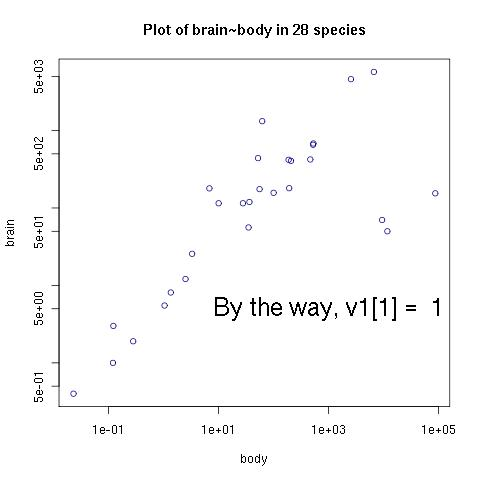
\includegraphics[height=5.5cm]{figs/plot.jpg}  
 \end{center}

\end{frame}

%%%%%%%%%%%%%%%%%%%%%%%%%%%%%%%%%%%%%%%%%%%%%%%%%%%%%%%%%%%%%%%%%%%%%%%

\begin{frame}[fragile]

 \frametitle{Plot least squares fit}
A.k.a. simple linear regression line.
 \begin{footnotesize}
\begin{verbatim}
> abline(lm(log10(Animals\$brain)~log10(Animals\$body)), col=``red'')
 \end{verbatim}
\end{footnotesize}
 \vspace{-0.7cm}
 \begin{center}
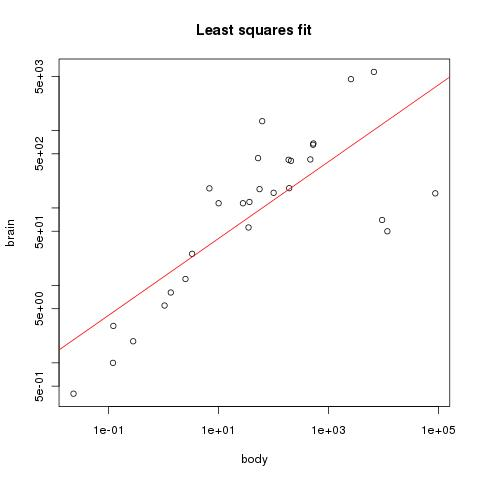
\includegraphics[height=5.5cm]{figs/lm.jpeg}  
 \end{center}

\end{frame}

%%%%%%%%%%%%%%%%%%%%%%%%%%%%%%%%%%%%%%%%%%%%%%%%%%%%%%%%%%%%%%%%%%%%%%%

\begin{frame}[fragile]
  
\frametitle{Histogram and Kernel Density Estiamtion}
 \begin{footnotesize}
   \begin{verbatim}
> hist(rnorm(n=5000, m=2, sd=2), freq=F, 
+ main = "Histogram and KDE of Gaussiand dist.")
> lines(rnorm(n=5000, m=2, sd=2), col="red", lwd=2, lty=2)
   \end{verbatim}
 \end{footnotesize}
\vspace{-1cm}
\begin{figure}
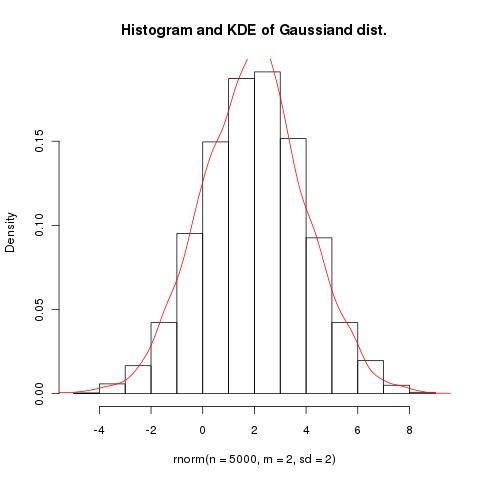
\includegraphics[height=5.5cm]{figs/hist.jpeg}
\end{figure}

\end{frame}

%%%%%%%%%%%%%%%%%%%%%%%%%%%%%%%%%%%%%%%%%%%%%%%%%%%%%%%%%%%%%%%%%%%%%%%

\begin{frame}

\frametitle{Resources}
 \begin{itemize}
  \item Multiplatform support: GNU/Linux, MacOS (and, yes... Windows, as well).
  \item Resources for GNU R in \textbf{R CRAN}:
  \url{http://cran.es.r-project.org/}. 
  \begin{enumerate}
   \item \textit{Packages}: browse the 
   complete list, descriptions, dependencies.
   \item Official manuals.
   \item Contributed manuals.
   \item FAQ lists.
  \end{enumerate}
 \end{itemize}

\end{frame}

%%%%%%%%%%%%%%%%%%%%%%%%%%%%%%%%%%%%%%%%%%%%%%%%%%%%%%%%%%%%%%%%%%%%%%%

\begin{frame}

 \frametitle{Good references for GNU R.}
 \begin{enumerate}
  \item Peter Dalgaard.\textit{Introductory Statistics with R}, 2nd ed., (2008). Springer.
  \item Maindonald \& Braun. \textit{Data Analysis and Graphics Using R}, 2nd ed., (2006).
  Cambridge University Press.
  \item Adler. \textit{R in a Nutshell}, (2010). O'Reilly Media.
  
 \end{enumerate}
 But...you should also know something about Statistics.
 \begin{itemize}
  \item Montgomery \& Runger. \textit{Applied Statistics and Probability for Engineers},
  4th ed, (2006). Wiley.
 \end{itemize}

\end{frame}

%%%%%%%%%%%%%%%%%%%%%%%%%%%%%%%%%%%%%%%%%%%%%%%%%%%%%%%%%%%%%%%%%%%%%%%

\begin{frame}

 \frametitle{Journals and web resources}
 \begin{enumerate}

  \item Journal of Statistical Software.
  \begin{itemize}
    \item \url{http://www.jstatsoft.org/}
  \end{itemize}

  \item The R Journal.
    \begin{itemize}
      \item Former R News, offers informative articles on libraries and
      new releases.
      \item \url{http://journal.r-project.org/}
    \end{itemize}

   \item Websites \& blogs.
    \begin{itemize}
      \item R-Forge (1,132 projects): \url{https://r-forge.r-project.org/}
      \item R blogs: \url{http://www.r-bloggers.com/blogs-list/}
    \end{itemize}

   \item R conferences.
     \begin{itemize}
      \item \url{http://www.r-project.org/conferences.html}
     \end{itemize}


 \end{enumerate}

\end{frame}

%%%%%%%%%%%%%%%%%%%%%%%%%%%%%%%%%%%%%%%%%%%%%%%%%%%%%%%%%%%%%%%%%%%%%%%

\end{document}

